\documentclass{article}

\usepackage{amsmath, mathrsfs, amssymb, stmaryrd, cancel, relsize,tikz,amsthm,comment,enumerate}

\theoremstyle{definition}
\newtheorem{Q}{Question}

\newcommand{\tvs}{\textvisiblespace}
\newcommand{\ra}{\rightarrow}
\newcommand{\la}{\leftarrow}
%\includecomment{comment}

%\pagenumbering{gobble}

\title{ITCS 532 Foundations of Computer Science\\
Week 1 - Models of Computation (Homework)}
\author{Rob Egrot}
\date{}

\begin{document}
\maketitle

\begin{Q}
A quadratic in $x$ over the integers has form $q(x)=ax^2+bx+c$, where $x$ is a variable and $a,b$ and $c$ are integers. Suppose our decision problem is whether a given quadratic over the integers has a root in the integers. So the set of instances is the set of all quadratics over the integers. A quadratic $q$ is a yes instance if there is an integer $z$ such that $q(z)=0$.

Design a suitable encoding system for this decision problem (you don't need to design a Turing machine to solve it!).
\end{Q}
\begin{comment}
\textbf{Solution}
Use $\Sigma = \{1,-,*\}$. Store $a$, $b$ and $c$ in unary, separated by $*$, using $-$ to denote negatives. E.g. we express $2x^2 - 3x +1$ as $11*-111*1$.
\end{comment}

\begin{Q}
Let $\Sigma=\{1,*\}$. Design a Turing machine that accepts as input a unary number (i.e. a finite string containing only 1s), and outputs that number multiplied by 2. E.g. If the input is 111 the output will be 111111. Hint: $*$ does not appear in the input or the output, but we can use it during the process of calculating the output.
\end{Q}
\begin{comment}
\textbf{Solution}
\begin{center}
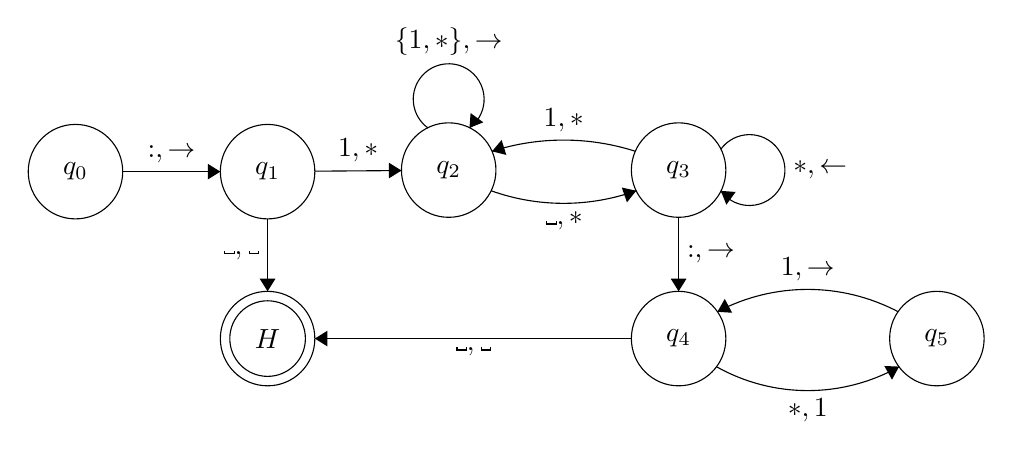
\begin{tikzpicture}[scale=0.2]
\tikzstyle{every node}+=[inner sep=0pt]
\draw [black] (14.6,-15.2) circle (3);
\draw (14.6,-15.2) node {$q_0$};
\draw [black] (26.8,-15.2) circle (3);
\draw (26.8,-15.2) node {$q_1$};
\draw [black] (26.8,-25.8) circle (3);
\draw (26.8,-25.8) node {$H$};
\draw [black] (26.8,-25.8) circle (2.4);
\draw [black] (38.3,-15.1) circle (3);
\draw (38.3,-15.1) node {$q_2$};
\draw [black] (52.9,-15.1) circle (3);
\draw (52.9,-15.1) node {$q_3$};
\draw [black] (52.9,-25.8) circle (3);
\draw (52.9,-25.8) node {$q_4$};
\draw [black] (69.3,-25.8) circle (3);
\draw (69.3,-25.8) node {$q_5$};
\draw [black] (17.6,-15.2) -- (23.8,-15.2);
\fill [black] (23.8,-15.2) -- (23,-14.7) -- (23,-15.7);
\draw (20.7,-14.7) node [above] {$:,\ra$};
\draw [black] (26.8,-18.2) -- (26.8,-22.8);
\fill [black] (26.8,-22.8) -- (27.3,-22) -- (26.3,-22);
\draw (26.3,-20.5) node [left] {$\tvs,\tvs$};
\draw [black] (29.8,-15.17) -- (35.3,-15.13);
\fill [black] (35.3,-15.13) -- (34.5,-14.63) -- (34.5,-15.63);
\draw (32.55,-14.63) node [above] {$1,\ast$};
\draw [black] (36.977,-12.42) arc (234:-54:2.25);
\draw (38.3,-7.85) node [above] {$\{1,\ast\},\ra$};
\fill [black] (39.62,-12.42) -- (40.5,-12.07) -- (39.69,-11.48);
\draw [black] (50.209,-16.412) arc (-70.28917:-109.71083:13.666);
\fill [black] (50.21,-16.41) -- (49.29,-16.21) -- (49.62,-17.15);
\draw (45.6,-17.71) node [below] {$\tvs,\ast$};
\draw [black] (55.58,-13.777) arc (144:-144:2.25);
\draw (60.15,-15.1) node [right] {$\ast,\la$};
\fill [black] (55.58,-16.42) -- (55.93,-17.3) -- (56.52,-16.49);
\draw [black] (52.9,-18.1) -- (52.9,-22.8);
\fill [black] (52.9,-22.8) -- (53.4,-22) -- (52.4,-22);
\draw (53.4,-20.45) node [right] {$:,\ra$};
\draw [black] (66.899,-27.585) arc (-60.64203:-119.35797:11.828);
\fill [black] (66.9,-27.58) -- (65.96,-27.54) -- (66.45,-28.41);
\draw (61.1,-29.6) node [below] {$\ast,1$};
\draw [black] (55.359,-24.095) arc (117.75844:62.24156:12.326);
\fill [black] (55.36,-24.1) -- (56.3,-24.16) -- (55.83,-23.28);
\draw (61.1,-22.18) node [above] {$1,\ra$};
\draw [black] (49.9,-25.8) -- (29.8,-25.8);
\fill [black] (29.8,-25.8) -- (30.6,-26.3) -- (30.6,-25.3);
\draw (39.85,-26.3) node [below] {$\tvs,\tvs$};
\draw [black] (41.046,-13.906) arc (107.74904:72.25096:14.937);
\fill [black] (41.05,-13.91) -- (41.96,-14.14) -- (41.66,-13.19);
\draw (45.6,-12.69) node [above] {$1,\ast$};
\end{tikzpicture}
\end{center}
\end{comment}

\begin{Q}
Can a formal language $L$ exist that is recursive but not r.e.?
\end{Q}
\begin{comment}
\textbf{Solution}
No. We know from the notes that decidable implies semidecidable, and this is just the formal language version of that.
\end{comment}

\begin{Q}
Suppose we define a class $\mathcal C$ of abstract computational devices similar to Turing machines but without the $\la$ command (so the tape head may never move backwards).
\begin{enumerate}[(a)]
\item Give an informal argument for why this model of computation is strictly weaker than that of Turing machines.
\item Would it make any difference if we replaced the $\la$ command with a $-$ command that keeps the tape head in the same place?
\item (Hard) Give a rigorous proof for part (a).
\end{enumerate}
\end{Q}
\begin{comment}
\textbf{Solution}
\begin{enumerate}[(a)]
\item No memory.
\item No. Still no memory. 
\item Consider the problem of checking to see if two strings are the same length. Input is, for example, a string of $1$'s followed by a $*$, followed by another string of $1$'s. Suppose we have a $-$ machine $M$ that solves this problem. Then it has a finite number of states, $n$ say. Consider the set $X$ that contains all strings of $k$ ones followed by a $*$, for $k\in\{1,\ldots,n+1\}$. Since $M$ cannot move its tape head backwards, the state it's in when it gets to the $*$ symbol must store all the information about the length of the first string. As $|X| = n+1$, by the pigeon hole principle there must be (at least) two strings in $X$ such that $M$ is in the same state when it gets to $*$. Call these strings $s*$ and $t*$. Then $M$ should accept $s*s$, but then it must also accept $t*s$, which is incorrect. 
\end{enumerate}
\end{comment}

\end{document}